\section{Gradient Descent with Large Datasets}
\subsection{Stochastic gradient descent}
\begin{itemize}
    \item \textbf{Batch gradient decent}:  In each iteration, sum cost of all \emph{m} examples, then taking one step of minimization (improving parameters). Might be expensive as number (of training examples) scales up.
    \item \textbf{Stochastic gradient descent}: take single cost of a training example, start improving the parameters towards global minimum. The algorithm may not converge immediately in a direct path; the route taken might be conservative and biased towards each individual sample. Might not converge to a single minimum; algorithm might end up wandering near the minimum-- this is a "good enough" hypothesis in most cases. Usually 1-10 iterations.
    \item \textbf{Mini-batch gradient descent}: use \emph{b} examples in each iteration (rather than all m). Step in size of \emph{b}. Also faster than Batch gradient descent. Outperforms Stochastic gradient descent if good vectorization can be performed (achieve parallelism). Downside: extra variable b.
\end{itemize}
\subsection{Stochastic gradient descent convergence and tuning}
\par Recall for Batch gradient descent, we had to plot $J_{train} (\theta)$ as a function of number of iterations of gradient descent. 

\par For Stochastic gradient descent, during learning, compute $cost(\theta, (x^{(i)}, y^{(i)}))$ before updating $\theta$ using $(x^{(i)}, y^{(i)})$. For every 1000 iterations, plot averaged over last 1000 examples. This gives a running estimate of how well minimization performs. IF we see that the running estimate increases over time, we can try to use a smaller learning rate $\alpha$; each iteration of the stochastic gradient descent will take a smaller step, thereby increasing the likelihood of convergence. 





\subsection{Advanced topic: online learning}
\begin{itemize}
    \item Take one example, improve parameters based on the single example (this is essentially stochastic gradient descent). Discard example. 
    \item Useful when website gets a stream of data from different users. 
    \item Can adapt to varying user preference.
    \item Search query keywords (Predicted CTR Click-through-rate): $p(y=1 | x;\theta)$.
\end{itemize}
\subsection{Advanced topic: map reduce and data parallelism}
\begin{itemize}
    \item Split examples into batches for different machines. 
    \item Each machine will compute semi-total cost according to the batch it was assigned. 
    \item Combine calculated cost to perform gradient descent and get a single $\theta$.
    \item Net result is equivalent to original 
    \item Applicable to multi-core machines: no network latency.
\end{itemize}

\begin{figure}[htpb]
    \centering
    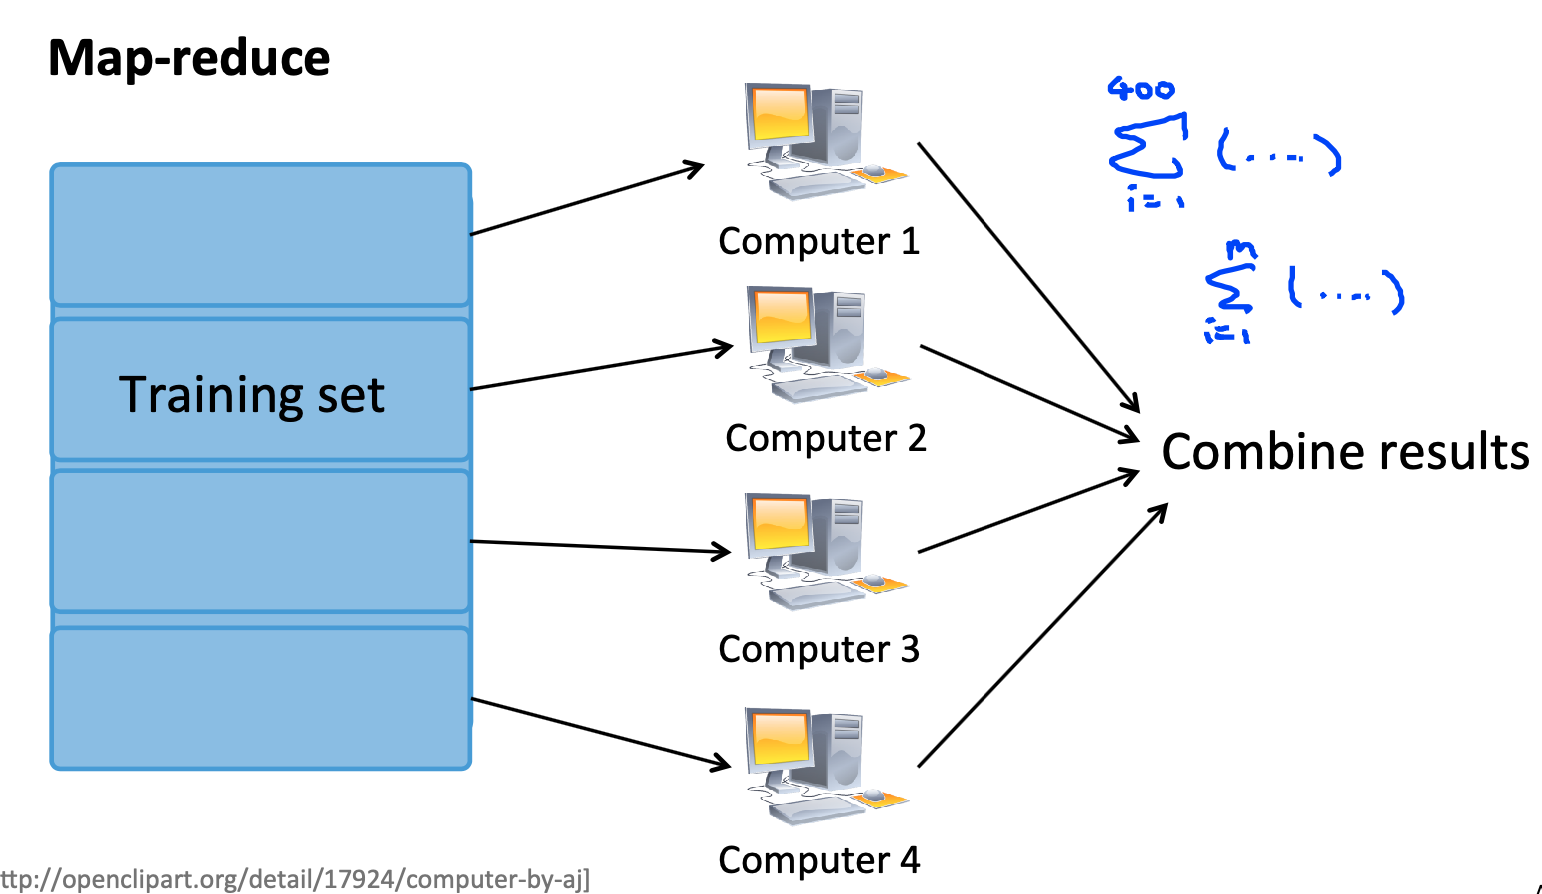
\includegraphics[width=0.8\textwidth]{image/map-reduce.png}
    \caption{Map reduce}
    \label{fig:map-reduce}
\end{figure}

\subsection{Stochastic gradient descent applications}
\par Many learning algorithms can be expressed as computing sums of functions over the training set; map-reduce is good candidate for such algorithms, where the bottleneck stems from summing over the training set. Because of network latency and other overhead, if we run map-reduce on N computers, we might get less than an N-fold speedup.
\begin{itemize}
    \item Batch gradient descent: split dataset into N smaller batches, compute the gradient for each smaller batch on each machine, then average the gradients on a central computer for the gradient update. This works for regressions and neural network training
    \item Stochastic gradient descent: \textbf{Not applicable}. Since stochastic gradient descent processes one example at a time and performs update after each example, it cannot be easily parallelized.
\end{itemize}


